%%%%%%%%%%%%%%%%%%%%%%%%%%%%%%%%%%%%%%%%%%%%%%%%%%%%%%%%%%%%%%%%%%%%%%
%
% AQIS extended abstract generated from
% Entanglement_enhanced_resilience(SA).tex
%
%%%%%%%%%%%%%%%%%%%%%%%%%%%%%%%%%%%%%%%%%%%%%%%%%%%%%%%%%%%%%%%%%%%%%%

\documentclass[a4paper]{article}
\usepackage{aqis}
\usepackage{graphicx}

\graphicspath{{../Figures/}{Figures/}}

\newcommand{\ket}[1]{\left|#1\right\rangle}
\newcommand{\bra}[1]{\left\langle #1\right|}
\newcommand{\norm}[1]{\left\lVert #1\right\rVert}
\newcommand{\Tr}{\operatorname{Tr}}
\DeclareMathOperator{\support}{supp}

\begin{document}

\title{
Entanglement-Induced Resilience in Analog Simulation and Quantum Control
}

\author{
Tianfeng~Feng\affiliation{1},
Yue~Cao\affiliation{1},
Wenjun~Yu\affiliation{1},
Junkai~Zeng\affiliation{2}\\
Xiaopeng~Li\affiliation{3}\email{xiaopeng\_li@fudan.edu.cn},
Xiu-Hao~Deng\affiliation{2}\affiliation{4}\email{dengxiuhao@iqasz.cn},
Qi~Zhao\affiliation{1}\affiliation{2}\email{zhaoqi@cs.hku.hk}
}

\address{1}{
QICI Quantum Information and Computation Initiative, Department of Computer Science,
The University of Hong Kong, Pokfulam Road, Hong Kong SAR, China
}
\address{2}{
Shenzhen International Quantum Academy, Shenzhen 518048, China
}
\address{3}{
State Key Laboratory of Surface Physics, Key Laboratory of Micro and Nano
Photonic Structures (MOE), and Department of Physics, Fudan University,
Shanghai 200433, China
}
\address{4}{
Shenzhen Branch, Hefei National Laboratory, Shenzhen 518048, China
}

\abstract{
We identify and numerically demonstrate entanglement-induced resilience in
realistic quantum dynamics. Our main evidence comes from three application
settings: analog simulation of spin models, analog simulation of fermionic
models, and quantum-control protocols. Across extensive simulations of
transverse-field Ising systems, Fermi-Hubbard lattices, and quantum-dot gate
control, states that generate larger subsystem entanglement consistently show
smaller coherent dynamical errors. Theoretically, local perturbative errors
are bounded by a Frobenius-norm contribution plus entropy-dependent
corrections, explaining why highly entangled dynamics approaches average-case
rather than worst-case behavior. These results suggest a practical route to
more robust analog simulators and control protocols.
}

\keywords{analog quantum simulation, fermionic simulation, quantum control, entanglement}

\maketitle

\section{Introduction}

Analog quantum simulators and quantum-control devices are built from
interacting many-body systems, and their dominant errors are often coherent:
static disorder, imperfect couplings, crosstalk, pulse distortions, and
spectator-induced shifts. Such errors are hard to remove completely, especially
in near-term devices where full quantum error correction is unavailable. Our
work asks whether the many-body dynamics itself can reduce sensitivity to
these perturbations.

The central answer is that dynamically generated entanglement can provide a
native resilience mechanism. The main contribution of this work is not only a
general bound, but a set of numerical demonstrations in three experimentally
motivated settings: spin-model analog simulation, fermionic analog simulation,
and quantum control. In each setting, we compare high-entanglement and
low-entanglement dynamical regimes and observe the same behavior: larger
subsystem entanglement suppresses coherent dynamical error.

\section{Theory}

Let $H_0(t)$ generate the ideal evolution $U_0(t)$ and let the implemented
dynamics be generated by
\[
  \widetilde{H}(t)=H_0(t)+H_{\rm pert}(t),
\]
where $H_{\rm pert}$ contains disorder and systematic imperfections. For an
initial state $\ket{\psi}$, the state-dependent error obeys
\begin{equation}
 \norm{(U_0(t)-U(t))\ket{\psi}}
 \leq \int_0^t d\tau\,
 \norm{H_{\rm pert}(\tau)\ket{\psi(\tau)}} ,
\label{eq:basic-bound}
\end{equation}
where $\ket{\psi(\tau)}=U_0(\tau)\ket{\psi}$. Therefore, the relevant error is
not only the operator norm of the perturbation, but also its action on the
actual evolved state.

For local perturbations $H_{\rm pert}=\sum_jH_j$, this action is controlled by
local entanglement. If $A=\sum_jA_j$ is positive semidefinite and local, then
\begin{equation}
 \bra{\psi}A\ket{\psi}
 \leq \frac{\Tr(A)}{d}
 +\sum_j\norm{A_j}
 \sqrt{2\log d_{\support(A_j)}-2S(\rho_j)} ,
\label{eq:entropy-bound}
\end{equation}
where $\rho_j$ is the reduced state on the support of $A_j$. Applying this to
$A=H_{\rm pert}^{\dagger}H_{\rm pert}$ shows that highly entangled subsystems
drive the entropy-dependent correction toward zero, leaving the normalized
Frobenius scale $\norm{H_{\rm pert}}_F$. Thus entanglement changes the relevant
scaling from worst-case spectral-norm behavior to average-case
Frobenius-norm behavior.

\section{Application I: Spin Models}

Our first and most direct numerical test is analog simulation of spin systems.
We study the one-dimensional transverse-field Ising model
\[
 H_0=h_x\sum_i X_i+h_y\sum_iY_i+J\sum_iX_iX_{i+1},
\]
with $h_x=0.809$, $h_y=0.9045$, and $J=1$. The imperfect simulator includes
both local disorder, $H_{\rm dis}=\sum_i\delta_iX_i$, and systematic coupling
imperfection, $H_{\rm imp}=\eta\sum_iX_iX_{i+1}$.

The numerical results show a clear separation between typical and atypical
input states. For $\ket{0}^{\otimes N}$, the dynamics rapidly generates
subsystem entanglement; after this growth, the simulation error follows the
Frobenius-norm prediction. For $\ket{+}^{\otimes N}$, entanglement remains
small and the error stays much closer to the spectral-norm bound. We also
evaluate one-segment simulation errors along the trajectory and find that
local entropy growth is accompanied by error suppression. Additional spin
simulations in two-dimensional settings show the same trend.

\begin{figure}[t]
\centering
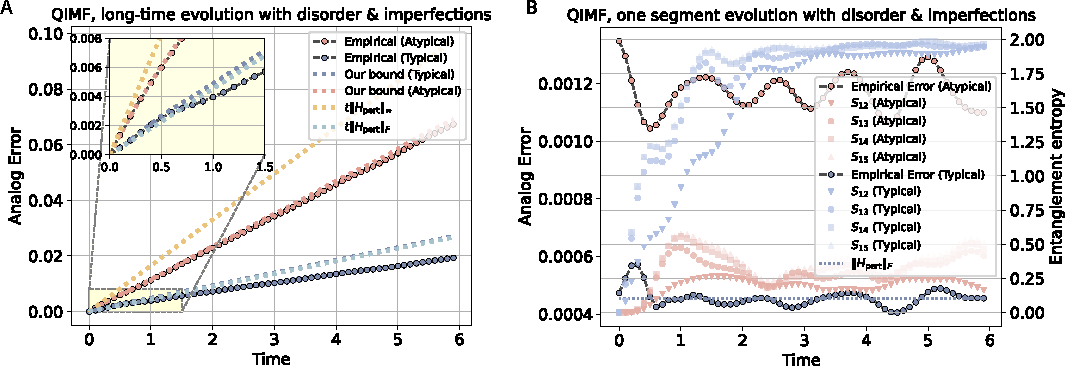
\includegraphics[width=0.98\columnwidth]{fig2.pdf}
\caption{\textbf{Spin-model analog simulation.}
In the transverse-field Ising model, high-entanglement dynamics follows the
Frobenius-norm estimate, while low-entanglement dynamics remains closer to
the worst-case spectral-norm behavior.}
\label{fig:spin}
\end{figure}

\section{Application II: Fermionic Models}

The second application is analog simulation of fermionic systems, where the
many-body Hilbert space and conservation laws differ substantially from spin
models. We study Fermi-Hubbard dynamics with periodic boundary conditions,
\[
H_0=-\sum_{i,\sigma}(a_{i,\sigma}^{\dagger}a_{i+1,\sigma}+{\rm H.c.})
 +V\sum_i n_{i,\uparrow}n_{i,\downarrow},
\]
and perturb the simulator by an additional Coulomb term
\[
H_{\rm pert}=\delta\sum_i n_{i,\uparrow}n_{i,\downarrow}.
\]

We compute segment-level errors with $\Delta t=0.1$ for several initial
fermionic configurations. The results again show a robust inverse correlation:
when two-site subsystem entanglement approaches its maximum, the empirical
simulation error drops toward the Frobenius estimate; when entanglement
decreases, the error develops sharp spikes. This behavior appears in both
one-dimensional and two-dimensional Fermi-Hubbard simulations, indicating that
entanglement-induced resilience is not an artifact of Pauli spin dynamics.

\begin{figure}[t]
\centering
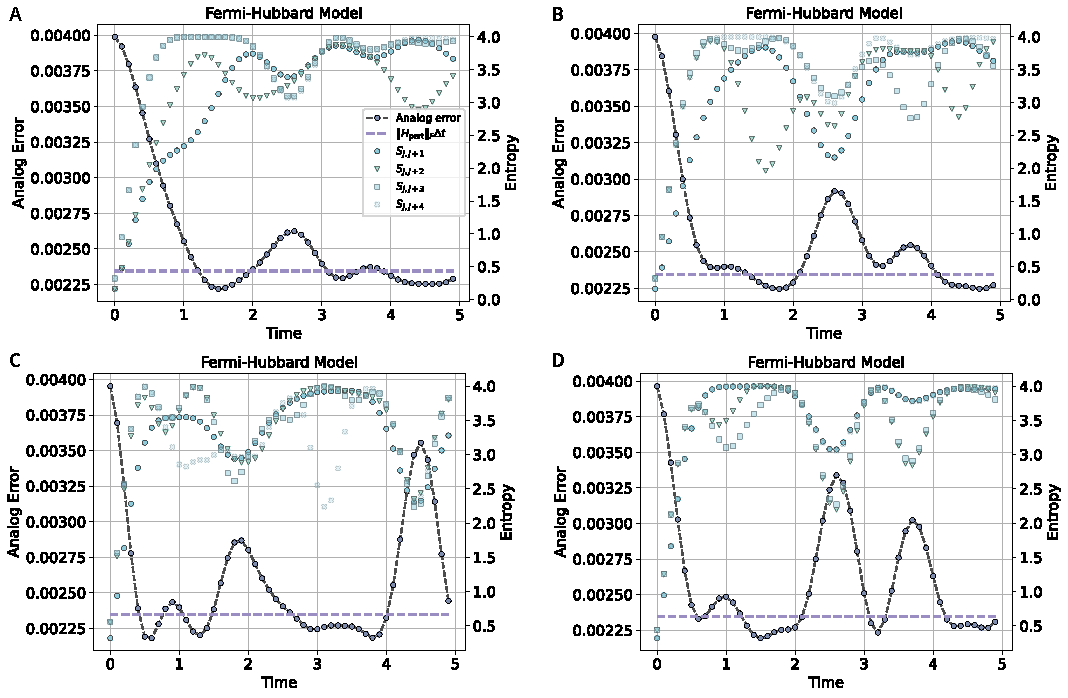
\includegraphics[width=0.98\columnwidth]{fig3.pdf}
\caption{\textbf{Fermionic analog simulation.}
In Fermi-Hubbard simulations, segment errors decrease as the relevant
two-site entanglement entropy increases, and error spikes occur when the
entropy drops.}
\label{fig:fermi}
\end{figure}

\section{Application III: Quantum Control}

The third application is real-time quantum control. We consider a target gate
implemented in a larger register, where nearby spectator qubits couple to the
driven qubit and create unavoidable coherent perturbations. For a target
subsystem $A$ consisting of the driven qubit and nearby spectators, our bound
predicts that entanglement between $A$ and the rest of the register reduces
the effective gate error toward the Frobenius scale of the time-dependent
perturbation.

We test this prediction in a $3\times4$ quantum-dot array using robust control
pulses for $X_\pi$, $X_{\pi/2}$, and $X_{2\pi}$ gates. The perturbation model
includes frequency drift, residual couplings, and pulse-amplitude errors. To
scan different entanglement regimes, we use purified Gibbs states whose
temperature controls the entanglement entropy between the target neighborhood
and the rest of the array. In all tested gates, the effective error decreases
rapidly as this entropy approaches its maximum. This shows that entanglement
can improve gate robustness even on top of optimized robust-control pulses.

\begin{figure}[t]
\centering
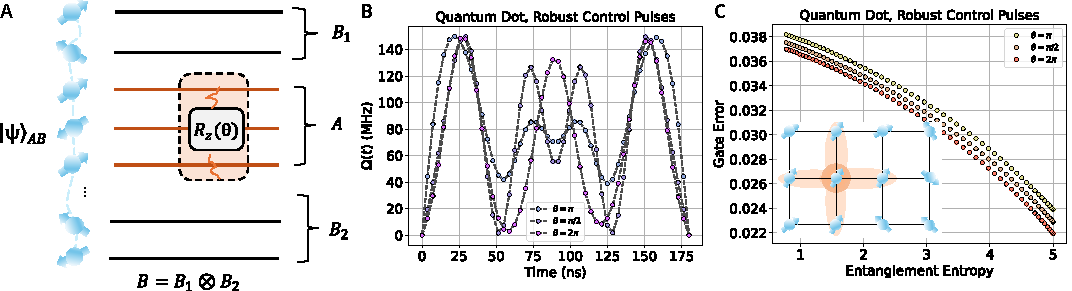
\includegraphics[width=0.98\columnwidth]{fig5.pdf}
\caption{\textbf{Quantum-control protocols.}
For robustly driven quantum-dot gates, larger entanglement between the target
neighborhood and the rest of the register correlates with lower effective
gate error.}
\label{fig:control}
\end{figure}

\section{Diagnostics and Outlook}

The numerical studies also suggest a practical diagnostic. Even when the
precise coefficients of $H_{\rm pert}$ are unknown, the local structure of
dominant noise terms is often known from the device layout. Measuring
coefficient-independent cross-term correlators,
\[
\frac{\bra{\psi(t)}H_j^\dagger H_{j'}+{\rm H.c.}\ket{\psi(t)}}
{\norm{H_j}\norm{H_{j'}}},
\]
can indicate whether the relevant local reduced states are close to maximally
mixed. In our spin-model tests, typical high-entanglement states yield many
near-zero cross terms, while atypical low-entanglement states yield sizable
correlations.

Taken together, the spin-model, fermionic-model, and quantum-control
experiments support a unified picture: entanglement growth can make coherent
perturbations act like average-case errors rather than worst-case errors. This
provides concrete guidance for designing analog simulators and control
protocols: engineer dynamics that generate entanglement on the supports where
dominant perturbations act.

\begin{thebibliography}{9}

\bibitem{Buluta09}
I.~Buluta and F.~Nori.
\newblock Quantum simulators.
\newblock {\em Science}, 326:108--111, 2009.

\bibitem{Daley22}
A.~J. Daley et al.
\newblock Practical quantum advantage in quantum simulation.
\newblock {\em Nature}, 607:667--676, 2022.

\bibitem{Lloyd96}
S.~Lloyd.
\newblock Universal quantum simulators.
\newblock {\em Science}, 273:1073--1078, 1996.

\bibitem{Childs21}
A.~M. Childs, Y.~Su, M.~C. Tran, N.~Wiebe, and S.~Zhu.
\newblock Theory of Trotter error with commutator scaling.
\newblock {\em Phys. Rev. X}, 11:011020, 2021.

\bibitem{Abanin19}
D.~A. Abanin, E.~Altman, I.~Bloch, and M.~Serbyn.
\newblock Colloquium: Many-body localization, thermalization, and entanglement.
\newblock {\em Rev. Mod. Phys.}, 91:021001, 2019.

\bibitem{Preskill12}
J.~Preskill.
\newblock Quantum computing and the entanglement frontier.
\newblock arXiv:1203.5813, 2012.

\bibitem{Hauke16}
P.~Hauke, M.~Heyl, L.~Tagliacozzo, and P.~Zoller.
\newblock Measuring multipartite entanglement through dynamic susceptibilities.
\newblock {\em Nat. Phys.}, 12:778--782, 2016.

\bibitem{Cottrell19}
W.~Cottrell, B.~Freivogel, D.~M. Hofman, and S.~F. Lokhande.
\newblock How to build the thermofield double state.
\newblock {\em J. High Energy Phys.}, 2019:058, 2019.

\end{thebibliography}

\end{document}
